\hypertarget{multiple-control-variables}{}
\section{Multiple Control Variables}\label{sec:multiple-control-variables}
We now consider how to solve problems with multiple control variables.  

\subsection{Theory}\label{subsec:MCTheory}

The new portfolio-share control variable is captured by the archaic Greek character \href{https://en.wikipedia.org/wiki/Stigma_(ligature)}{`stigma'}; it represents the share $\Shr$ of their disposable assets the agent invests in the risky asset (conventionally, the stock market).  Designating the return factor for the risky asset as $\Risky$ and the share of the portfolio invested in $\Risky$ as $\Shr$, the realized portfolio rate of return $\Rport$ as a function of the share $\Shr$ is:
\begin{equation}\begin{gathered}\begin{aligned}
      \Rport(\Shr) &= \Rfree+(\Risky-\Rfree)\Shr \label{eq:Shr}.
    \end{aligned}\end{gathered}\end{equation}
If we imagine the portfolio share decision as being made simultaneously with the $\cNrm$ decision, the traditional way of writing the problem is (substituting the budget constraint):
\begin{equation}\begin{gathered}\begin{aligned}
      \vFunc_{\prd}(m)  & = \max_{\{\cFunc,\Shr\}} ~~  \uFunc(c) + \ExMidStg[\DiscFac \vFunc_{\prd+1}((m-c)\Rport(\Shr) + {\TranShkEmp}_{\prd+1})] \label{eq:Bellmanundated}
    \end{aligned}\end{gathered}\end{equation}
where we have deliberately omitted the {\interval}-designating subscripts for $\Shr$ and the return factors to highlight the point that, once the consumption and $\Shr$ decisions have been made, it makes no difference to this equation whether the risky return factor $\Risky$ is revealed a nanosecond before the end of the current {\interval} or a nanosecond after the beginning of the successor {\interval}.


\begin{comment}
  Designating the return factor for the risky asset as $\Risky_{\prd+1}$, and using $\Shr_{\prd}$ to represent the proportion of the portfolio invested in this asset before the return is realized after the beginning of $\prd+1$, corresponding to an assumption that the consumer cannot be `net short' and cannot issue net equity), the overall return on the consumer's portfolio between $t$ and $t+1$ will be:
    \begin{equation}\begin{gathered}\begin{aligned}
          \Rport_{\prd+1}  & = \Rfree(1-\Shr_{\prd}) + \Risky_{\prd+1}\Shr_{\prd} \label{eq:return1}
          \\               & = \Rfree + (\Risky_{\prd+1}-\Rfree) \Shr_{\prd} %\label{eq:return2}
        \end{aligned}\end{gathered}\end{equation}
  and the maximization problem is
    \begin{equation*}\begin{gathered}\begin{aligned}
          \vFunc_{\prd}(m_{\prd})  & = \max_{\{{c}_{\prd},\Shr_{\prd}\}}   ~~ \uFunc(c_{\prd}) +  \DiscFac
          \ExEndStg[{\vFunc}_{\prd+1}(m_{\prd+1})]
          \\      & \text{s.t.} \nonumber
          \\      \Rport_{\prd+1}  & = \Rfree + (\Risky_{\prd+1}-\Rfree) \Shr_{\prd}
          \\      m_{\prd+1}  & = (m_{\prd}-c_{\prd})\Rport_{\prd+1} + \TranShkEmp_{\prd+1}
          \\  0       \leq & \Shr_{\prd}  \leq 1, \label{eq:noshorts}
        \end{aligned}\end{gathered}\end{equation*}

  The first order condition with respect to $c_{\prd}$ is almost identical to that in the single-control problem, equation (\ref{eq:upceqEvtp1}); the only difference is that the nonstochastic interest factor $\Rfree$ is now replaced by the portfolio return ${\Rport}_{\prd+1}$,
    \begin{equation}\begin{gathered}\begin{aligned}
          \uFunc^{c}(c_{\prd})  & = \DiscFac \ExEndStg [{\Rport}_{\prd+1} \vFunc^{m}_{\prd+1}(m_{\prd+1})] \label{eq:valfuncFOCRtilde},
        \end{aligned}\end{gathered}\end{equation}
  and the Envelope theorem derivation remains the same, yielding the Euler equation for consumption
    \begin{equation}\begin{gathered}\begin{aligned}
          \uFunc^{c}(c_{\prd})  & = \ExEndStg[\DiscFac {\Rport}_{\prd+1} \uFunc^{c}(c_{\prd+1})]. \label{eq:EulercRiskyR}
        \end{aligned}\end{gathered}\end{equation}

  The first order condition with respect to the risky portfolio share is
    \begin{equation}\begin{gathered}\begin{aligned}
          0  & = \ExEndStg[{\vFunc}_{\MidStgNxt}^{m}(m_{\prd+1})(\Risky_{\prd+1}-\Rfree){a}_{\prd}] \notag
          \\         & = \ExEndStg\left[\uFunc^{c}\left(\cFunc_{\prd+1}(m_{\prd+1})\right)(\Risky_{\prd+1}-\Rfree)\right]{a}_{\prd} 
          \\         & = \ExEndStg\left[\uFunc^{c}\left(\cFunc_{\prd+1}(m_{\prd+1})\right)(\Risky_{\prd+1}-\Rfree)\right], \label{eq:FOCw}        
        \end{aligned}\end{gathered}\end{equation}
  where the last line follows because $0/a_{\prd}=0$.

  As before, we define $\vEnd$ as a function that yields the expected $t+1$ value of ending period $t$ with assets $a_{\prd}$.  However, now that there are two control variables, the expectation must be defined as a function of the chosen values of both of those variables, because expected end-of-period value will depend not just on how much the agent saves, but also on how the saved assets are allocated between the risky and riskless assets.  Thus we define
  \begin{equation*}\begin{gathered}\begin{aligned}
        \vMidStg(a_{\prd},\Shr_{\prd})  & = \DiscFac \vFunc_{\arvlStgShr}(m_{\prd+1})
      \end{aligned}\end{gathered}\end{equation*}
  which has derivatives
  \begin{equation}\begin{gathered}\begin{aligned}
        \vMidStg^a  & = \ExEndStg[\DiscFac {\Rport}_{\prd+1}\vFunc_{\prd+1}^{m}(m_{\prd+1})] = \ExEndStg[\DiscFac {\Rport}_{\prd+1}{\uFunc}_{\prd+1}^{c}(\cFunc_{\prd+1}(m_{\prd+1}))]
      \end{aligned}\end{gathered}\end{equation}
  \begin{equation}\begin{gathered}\begin{aligned}
        \vMidStg^{\Shr}  & = \ExEndStg[\DiscFac (\Risky_{\prd+1}-\Rfree){\vFunc}_{\prd+1}^{m}(m_{\prd+1})  ]a_{\prd} = \ExEndStg[\DiscFac (\Risky_{\prd+1}-\Rfree){\uFunc}_{\prd+1}^{c}(\cFunc_{\prd+1}(m_{\prd+1}))  ]a_{\prd} \notag
      \end{aligned}\end{gathered}\end{equation}
  implying that the first order conditions (\ref{eq:EulercRiskyR}) and
  (\ref{eq:FOCw}) can be rewritten
  \begin{equation}\begin{gathered}\begin{aligned}
        \uFunc^{c}(c_{\prd})  & = \vMidStg^{a}(m_{\prd}-c_{\prd},\Shr_{\prd}) \label{eq:FOCc}
      \end{aligned}\end{gathered}\end{equation}
  and 
  \begin{equation}\begin{gathered}\begin{aligned}
        0  & = \vFunc^{\Shr}_{\vMidStgStgShr}(a_{\prd},\Shr_{\prd}). \label{eq:FOCShr}
      \end{aligned}\end{gathered}\end{equation}
\end{comment}

\hypertarget{stages-within-a-period}{}
\subsection{{\Stg}s Within a {\Interval}}\label{subsec:stageswithin}

which we will call the `consumption {\stg} $\cFunc$' and the `portfolio {\stg} $\Shr$.'  These could come in either order in the {\interval}: We designate the `portfolio choice first, then consumption' version by $[\Shr,\cFunc]$ and the `consumption choice first, then portfolio' as $[\cFunc,\Shr]$.

In a problem with multiple {\stgs}, if we want to refer to a sub-{\move} of a particular {\stg} -- say, the {\Arrival} {\stg} of the portfolio {\stg} -- we simply add a {\stg}-indicator subscript (in square brackets) to the notation we have been using until now.  That is, the {\Arrival} {\stg} of the portfolio problem would be $\vFunc_{_\arvl[\Shr]}$.

\hypertarget{revised-consumers-problem}{}
\subsubsection{The (Revised) Consumer's Problem}\label{subsubsec:revised-consumers-problem}

A slight modification to the consumer's problem specified earlier is necessary to make the {\stg}s of the problem completely modular.  The difficulty with the earlier formulation is that it assumed that asset returns occurred in the middle {\move} of the consumption problem.  Our revised version of the consumption problem takes as its input state the amount of bank balances that have resulted from any prior portfolio decision.  The problem is therefore:
  \begin{equation}\begin{gathered}\begin{aligned}
 \vFunc_{[\cFunc]}(\mNrm) & =  \max_{\cNrm} ~~ \uFunc(\cNrm)+  \vFunc_{[\cFunc]_{_\cntn}}(\underbrace{\mNrm-\cNrm}_{\aNrm})             
\\    \vFunc_{_\arvl[\cFunc]}(\bNrm) & = \Ex_{_\arvl[\cFunc]}\left[\vFunc_{[\cNrm]}(\overbrace{\bNrm+\TranShkEmp}^{m})\right] \label{eq:vBalances}
      \end{aligned}\end{gathered}\end{equation}


\hypertarget{subsubsec:investors-problem}{}
\subsubsection{The Investor's Problem}\label{subsubsec:investors-problem}

Consider the standalone problem of an `investor' whose continuation-value function $\vFunc_{[\Shr]_\cntn}$ depends on how much wealth $\wlthAftr$ they end up after the realization of the stochastic $\Risky$ return.  The expected value that the investor will obtain from any combination of initial $\wlthBefr$ and their optimal choice of the portfolio share $\Shr$ is the expectation of the continuation-value function over the wealth that results from the portfolio choice:
\begin{equation}\begin{gathered}\begin{aligned}
  \vFunc_{_\arvl[\Shr]}(\wlthBefr)  = & \max_{\Shr}~ \Ex_{\BegStg[\Shr]}\left[\vFunc_{[\Shr]_{_\cntn}}\overbrace{\left(\Rport(\Shr){\wlthBefr}\right)}^{\wlthAftr}\right] \label{eq:vMidStgShr}
    \end{aligned}\end{gathered}\end{equation}
where we have omitted any {\interval} designator like $\prd$ for the {\interval} in which this problem is solved because, with the continuation-value function defined already as $\vFunc_{[\Shr]_\cntn}(\wlthAftr)$, the problem is self-contained.  The solution to this problem will yield an optimal $\Shr$ decision rule $\optml{\Shr}(\wlthBefr).$  Finally, we can specify the value of an investor `arriving' with $\wlthBefr$ as the expected value that will be obtained when the investor invests optimally, generating the \textit{ex ante} optimal stochastic portfolio return factor $\optml{\Rport}(\wlthBefr)=\Rport(\optml{\Shr}(\wlthBefr))$:
\begin{equation}\begin{gathered}\begin{aligned}
      \vFunc_{_\arvl[\Shr]}(\wlthBefr)  = & \Ex_{_\arvl}[\vFunc_{[\Shr]_\cntn}](\overbrace{\optml{\Rport}(\wlthBefr)}^{\wlthAftr})].
\end{aligned}\end{gathered}\end{equation}

The reward for all this notational investment is that it is now clear that \emph{exactly the same code} for solving the portfolio share problem can be used in two distinct problems: a `beginning-of-period-returns' model and an `end-of-period-returns' model.

\hypertarget{beginning-returns}{}
\subsubsection{The `beginning-of-period returns' Problem}\label{subsubsec:beginning-returns}
The beginning-returns problem effectively just inserts a portfolio choice that happens at a {\stg} immediately before the consumption {\stg} in the optimal consumption problem described in \eqref{eq:vBalances}, for which we had a beginning-of-{\stg} value function $\vFunc_{_\arvl[\cFunc]}(\bNrm)$.  The agent makes their portfolio share decision within the {\stg} but (obviously) before the risky returns $\Risky$ for the {\interval} have been realized.  So the problem's portfolio-choice {\stg} also takes $\kNrm$ as its initial state and solves the investor's problem outlined in section~\ref{subsubsec:investors-problem} above:
\begin{equation}\begin{gathered}\begin{aligned}
  \vFunc_{_\arvl[\Shr]}(\kNrm) & = \Ex_{[_\arvl\Shr]}[\vFunc_{[\Shr]_{_\cntn}}(\underbrace{\kNrm\optml{\Rport}}_{\bNrm})]
\\\vFunc_{[\Shr]_\cntn}(\bNrm)  & = \vFunc_{_\arvl[\cFunc]}(\bNrm)
    \end{aligned}\end{gathered}\end{equation}

Since in this setup bank balances have been determined before the consumption problems starts, we need to rewrite the consumption {\stg}  as a function of bank balances that will have resulted from the portfolio investment $\bNrm$, combined with the income shocks $\TranShkEmp$:
\begin{equation}\begin{gathered}\begin{aligned}
      \vFunc_{_\arvl[\cFunc]}(\bNrm) = & \max_{\cFunc}~ \uFunc(\cNrm) + \Ex_{_\arvl[\cFunc]}[\vFunc_{[\cFunc]_\cntn}(\underbrace{\overbrace{\bNrm+\TranShkEmp}^{\mNrm}-\cNrm}_{\aNrm})]
    \end{aligned}\end{gathered}\end{equation}
where, because the consumption {\stg} is the last {\stg} in the {\interval}, the continuatibon-value function for the $\cFunc$ {\stg} is just the continuation-value function for the period as a whole:
\begin{equation}\begin{gathered}\begin{aligned}
      \vFunc_{[\cFunc]_\cntn}(\aNrm) = & \vFunc_{\prd_\cntn}(\aNrm)
    \end{aligned}\end{gathered}\end{equation}
(and recall that $\vFunc_{\prd_\cntn}(\aNrm)$ is exogenously provided as an input to the {\interval}'s problem via the transition equation assumed earlier: $\vFunc_{\prd_\cntn}(\aNrm)=\DiscFac \vFunc_{_\arvl(\prd+1)}(a)$).

\subsubsection{The `end-of-period-returns' Problem}

If the portfolio share and risky returns are realized at the end of the {\interval}, we need to move the portfolio choice {\stg} to immediately before the point at which returns are realized (and after the $\cFunc$ choice has been made).  The problem is the same as the portfolio problem defined above, except that the input for the investment {\stg} is the assets remaining after the consumption choice: $\aNrm$.  So, the portfolio {\stg} of the problem is
\begin{equation}\begin{gathered}\begin{aligned}
  \vFunc_{_\arvl[\Shr]}(\aNrm) = & \Ex_{_\arvl[\Shr]}[\vFunc_{[\Shr]_{_\cntn}}(\underbrace{\aNrm\optml{\Rport}}_{\kNrm})] %= \Ex_{[\cFunc]_\arvl}[\vFunc_{}(\kNrm)]
    \end{aligned}\end{gathered}\end{equation}
where we are designating the post-realization result of the investment as $\kNrm$, and since the $\Shr$-{\stg} is the last {\stg} of the problem the end-of-{\stg} $\kNrm$ becomes the end-of-{\interval} $\kNrm_{\prd}.$ 

The `state transition' equation between $\prd$ and $\prd+1$ is simply $\bNrm_{t+1} = \kNrm_{\prd}$ and the continuation-value function transition is $\vFunc_{\prd_\cntn}(\kNrm) \mapsto \DiscFac \vFunc_{_\arvl(\prd+1)}(\kNrm)$ which reflects the above-mentioned point that there is no substantive difference between the two problems (their $\vFunc_{[\cFunc]}(\mNrm)$ value functions and $\cFunc(\mNrm)$ functions will be identical).

(Note that we are assuming that there will be only one consumption function in the period, so no {\stg} subscript is necessary to pick out `the consumption function'). 

\subsubsection{Numerical Solution}
we can solve it numerically for the optimal $\Shr$ at a vector of $\vctr{a}$ ({\aVecCode} in the code)  and then construct an approximated optimal portfolio share function $\Aprx{\optml{\Shr}}(a)$ as the interpolating function among the members of the $\{\vctr{a},\vctr{\Shr}\}$ mapping.  Having done this, we can now calculate a vector of values and marginal values that correspond to $\aVec$:
\begin{equation}\begin{gathered}\begin{aligned}
      \vctr{v}  & = \vFunc_{_\arvl[\Shr]}(\vctr{a}) \label{eq:vShrEnd}
\\      \vctr{v}^\aNrm  & = \vFunc^{\aNrm}_{_\arvl[\Shr]}(\vctr{a}).
    \end{aligned}\end{gathered}\end{equation}

With the $\vctr{v}^{\aNrm}$ approximation described in hand, we can construct our approximation to the consumption function using \emph{exactly the same EGM procedure} that we used in solving the problem \emph{without} a portfolio choice (see \eqref{eq:cGoth}):
\begin{equation}\begin{gathered}\begin{aligned}
      \vctr{c}  & \equiv  \left(\vctr{\vNrm}^{\aNrm}\right)^{-1/\CRRA} \label{eq:cVecPort},
    \end{aligned}\end{gathered}\end{equation}
which, following a procedure identical to that in the EGM subsection \ref{subsec:egm}, yields an approximated consumption function $\Aprx{\cFunc}_{\prd}(m)$.  Thus, again, we can construct the consumption function at nearly zero cost (once we have calculated $\vctr{v}^{a}$).

\hypertarget{the-point}{}

\subsubsection{The Point}\label{subsubsec:the-point}

The upshot is that all we need to do is change some of the transition equations and we can use the same solution code (both for the $\Shr$-stage and the $\cFunc$-stage) to solve the problem with either assumption (beginning-of-period or end-of-period) about the timing of portfolio choice.  There is even an obvious notation for the two problems: $\vFunc_{_\arvl\prd[\Shr{c}]}$ can be the {\interval}-arrival value function for the version where the portfolio share is chosen at the beginning of the period, and $\vFunc_{_\arvl\prd[{c}\Shr]}$ is {\interval}-arrival value for the the problem where the share choice is at the end.

What is the benefit of writing effectively the identical problem in two different ways?  There are several:
\begin{itemize}
\item It demonstrates that, if they are carefully constructed, Bellman problems can be ``modular''
  \begin{itemize}
  \item In a life cycle model one might want to assume that at at some ages agents have a portfolio choice and at other ages they do not. The consumption problem makes no assumption about whether there is a portfolio choice decision (before or after the consumption choice), so there would be zero cost of having an age-varying problem in which you drop in whatever choices are appropriate to the life cycle stage.
  \end{itemize}
\item It emphasizes the flexibilty of choice a modeler has to date variables arbitrarily.  In the specific example examined here, there is a strong case for preferring the beginning-returns specification because we typically think of productivity or other shocks at date $\prd$ affecting the agent's state variables before the agent makes that period's choices.  It would be awkward and confusing to have a productivity shock dated $\prd-1$ effectively applying for the problem being solved at $\prd$ (as in the end-returns specification)
\item It may help to identify more efficient solution methods
  \begin{itemize}
  \item For example, under the traditional formulation in equation \eqref{eq:Bellmanundated} it might not occur to a modeler that the endogenous gridpoints solution method can be used, because when portfolio choice and consumption choice are considered simultaneously the EGM method breaks down because the portfolio choice part of the problem is not susceptible to EGM solution.  But when the problem is broken into two simpler problems, it becomes clear that EGM can still be applied to the consumption problem even though it cannot be applied to the portfolio choice problem
  \end{itemize}
\end{itemize}

% % the problem needs to be altered to bring the {\move}s involving the realization of risky returns into {\interval} $\prd$; the variable with which the agent ends the period is now $\bNrm_{\prd}$ and to avoid confusion with the prior model in which we assumed $k_{\prd+1}={a}_{\prd}$ we will now define $\kappa_{\prd+1}={\bNrm}_{\prd}$.  The continuation-value function for the $[\Shr]$ {\stg} now becomes
% % \begin{equation}\begin{gathered}\begin{aligned}




\subsection{Application}\label{subsec:MCApplication}


In specifying the stochastic process for $\Risky_{\prd+1}$, we follow the common practice of assuming that returns are lognormally distributed, $\log \Risky \sim \Nrml(\eprem+\rfree-\sigma^{2}_{\risky}/2,\sigma^{2}_{\risky})$ where $\eprem$ is the equity premium over the thin returns $\rfree$ available on the riskless asset.\footnote{This guarantees that $\Ex[\Risky] = \EPrem/\Rfree$ is invariant to the choice of $\sigma^{2}_{\eprem}$; see \handoutM{LogELogNorm}.}

As with labor income uncertainty, it is necessary to discretize the rate-of-return risk in order to have a problem that is soluble in a reasonable amount of time.  We follow the same procedure as for labor income uncertainty, generating a set of $n_{\risky}$ equiprobable shocks to the rate of return; in a slight abuse of notation, we will designate the portfolio-weighted return (contingent on the chosen portfolio share in equity, and potentially contingent on any other aspect of the consumer's problem) simply as $\Rport_{i,j}$ (where dependence on $i$ is allowed to permit the possibility of nonzero correlation between the return on the risky asset and the $\TranShkEmp$ shock to labor income (for example, in recessions the stock market falls and labor income also declines).

The direct expressions for the derivatives of $\vEndStg$ are
\begin{equation}\begin{gathered}\begin{aligned}
      \vEndStg^{a}(a_{\prd},\Shr_{\prd})  & = \DiscFac \left(\frac{1}{n_{\risky} n_{\TranShkEmp}}\right)\sum_{i=1}^{n_{\TranShkEmp}}\sum_{j=1}^{n_{\risky} }\Rport_{i,j} \left(\cFunc_{\prd+1}(\Rport_{i,j}a_{\prd}+\TranShkEmp_{i})\right)^{-\CRRA}
      \\      \vEndStg^{\Shr}(a_{\prd},\Shr_{\prd})  & = \DiscFac \left(\frac{1}{n_{\risky} n_{\TranShkEmp}}\right)\sum_{i=1}^{n_{\TranShkEmp}}\sum_{j=1}^{n_{\risky} }(\Risky_{i,j}-\Rfree)\left(\cFunc_{\prd+1}(\Rport_{i,j}a_{\prd}+\TranShkEmp_{i})\right)^{-\CRRA}.
    \end{aligned}\end{gathered}\end{equation}

Writing these equations out explicitly makes a problem very apparent: For every different combination of $\{{a}_{\prd},\Shr_{\prd}\}$ that the routine wishes to consider, it must perform two double-summations of $n_{\risky} \times n_{\TranShkEmp}$ terms.  Once again, there is an inefficiency if it must perform these same calculations many times for the same or nearby values of $\{{a}_{\prd},\Shr_{\prd}\}$, and again the solution is to construct an approximation to the (inverses of the) derivatives of the $\vEndStg$ function.

Details of the construction of the interpolating approximations are given below; assume for the moment that we have the approximations $\Aprx{\vFunc}_{\EndStg}^{a}$ and $\Aprx{\vFunc}_{\EndStg}^{\Shr}$ in hand and we want to proceed.  As noted above in the discussion of \eqref{eq:Bellmanundated}, nonlinear equation solvers can find the solution to a set of simultaneous equations.  Thus we could ask one to solve
\begin{equation}\begin{gathered}\begin{aligned}
      c_{\prd}^{-\CRRA}  & = \Aprx{\vFunc}^{a}_{{\prd_\cntn}}(m_{\prd}-c_{\prd},\Shr_{\prd}) %\label{eq:FOCwrtcMultContr}
      \\      0  & = \Aprx{\vFunc}^{\Shr}_{{\prd_\cntn}}(m_{\prd}-c_{\prd},\Shr_{\prd}) \label{eq:FOCwrtw}
    \end{aligned}\end{gathered}\end{equation}
simultaneously for $\cNrm$ and $\Shr$ at the set of potential $m_{\prd}$ values defined in {\mVec}. However, as noted above, multidimensional constrained
maximization problems are difficult and sometimes quite slow to
solve.

There is a better way.  Define the problem

\begin{equation}\begin{gathered}\begin{aligned}
      \Opt{\vFunc}_{{\prd_\cntn}}(a_{\prd})  & = \max_{\Shr_{\prd}} ~~  \vEndStg(a_{\prd},\Shr_{\prd})
      \\      & \text{s.t.} \nonumber
      \\      0 \leq & \Shr_{\prd} \leq 1
    \end{aligned}\end{gathered}\end{equation}
where the tilde over $\Opt{\vFunc}(a)$ indicates that this is the $\vFunc$ that has been optimized with respect to all of the arguments other than the one still present ($a_{\prd}$).  We solve this problem for the set of gridpoints in \code{aVec} and use the results to construct the interpolating function $\Aprx{\Opt{\vFunc}}_{\prd}^{a}(a_{\prd})$.\footnote{A faster solution could be obtained by, for each element in \code{aVec}, computing $\vEndStg^{\Shr}(m_{\prd}-c_{\prd},\Shr)$ of a grid of values of $\Shr$, and then using an approximating interpolating function (rather than the full expectation) in the \texttt{FindRoot} command.  The associated speed improvement is fairly modest, however, so this route was not pursued.}  With this function in hand, we can use the first order condition from the single-control problem
\begin{equation*}\begin{gathered}\begin{aligned}
      c_{\prd}^{-\CRRA}  & = \Aprx{\Opt{\vFunc}}_{\prd}^{a}(m_{\prd}-c_{\prd})
    \end{aligned}\end{gathered}\end{equation*}
to solve for the optimal level of consumption as a function of $m_{\prd}$ using the endogenous gridpoints method described above.  Thus we have transformed the multidimensional optimization problem into a sequence of two simple optimization problems.

Note the parallel between this trick and the fundamental insight of dynamic programming: Dynamic programming techniques transform a multi-period (or infinite-period) optimization problem into a sequence of two-period optimization problems which are individually much easier to solve; we have done the same thing here, but with multiple dimensions of controls rather than multiple periods.

\hypertarget{implementation}{}
\subsection{Implementation}

Following the discussion from section \ref{subsec:MCTheory}, to provide a numerical solution to the problem
with multiple control variables, we must define expressions that capture the expected marginal value of end-of-period
assets with respect to the level of assets and the share invested in risky assets. This is addressed in ``Multiple Control Variables.''



% Having the \texttt{GothicMC} subclass available, we can proceed with implementing the steps laid out in section \ref{subsec:MCApplication} to solve the problem at hand. Initially, the two distributions that capture the uncertainty faced by consumers in this scenario are discretized. Subsequently, the \texttt{GothicMC} class is invoked with the requisite arguments to create an instance that includes the necessary functions to depict the first-order conditions of the consumer's problem. Following that, an improved grid of end-of-period assets is established.

% Here is where we can see how the approach described in section \ref{subsec:MCApplication} is reflected in the code.  For the terminal period, the optimal share of risky assets is determined for each point in \texttt{aVec\_eee}, and then the endogenous gridpoints method is employed to compute the optimal consumption level given that the share in the risky asset has been chosen optimally. It's worth noting that this solution takes into account the possibility of a binding artificial borrowing constraint. Lastly, the interpolation process is executed for both the optimal consumption function and the optimal share of the portfolio in risky assets. These values are stored in their respective dictionaries (\texttt{mGridPort\_life}, \texttt{cGridPort\_life}, and \texttt{ShrGrid\_life}) and utilized to conduct the recursive process outlined in the `Recursion' section, thus yielding the numerical solution for all earlier periods.

\hypertarget{results-with-multiple-controls}{}
\subsection{Results With Multiple Controls}\label{subsec:results-with-multiple-controls}

Figure~\ref{fig:PlotctMultContr} plots the $\prd-1$ consumption function generated by the program; qualitatively it does not look much different from the consumption functions generated by the program without portfolio choice.

But Figure~\ref{fig:PlotRiskySharetOfat} which plots the optimal portfolio share as a function of the level of assets, exhibits several interesting features.  First, even with a coefficient of relative risk aversion of 6, an equity premium of only 4 percent, and an annual standard deviation in equity returns of 15 percent, the optimal choice is for the agent to invest a proportion 1 (100 percent) of the portfolio in stocks (instead of the safe bank account with riskless return $\Rfree$) is at values of $a_{\prd}$ less than about 2.  Second, the proportion of the portfolio kept in stocks is \textit{declining} in the level of wealth - i.e., the poor should hold all of their meager assets in stocks, while the rich should be cautious, holding more of their wealth in safe bank deposits and less in stocks.  This seemingly bizarre (and highly counterfactual -- see \cite{carroll:richportfolios}) prediction reflects the nature of the risks the consumer faces.  Those consumers who are poor in measured financial wealth will likely derive a high proportion of future consumption from their labor income.  Since by assumption labor income risk is uncorrelated with rate-of-return risk, the covariance between their future consumption and future stock returns is relatively low.  By contrast, persons with relatively large wealth will be paying for a large proportion of future consumption out of that wealth, and hence if they invest too much of it in stocks their consumption will have a high covariance with stock returns.  Consequently, they reduce that correlation by holding some of their wealth in the riskless form.

\hypertarget{PlotctMultContr}{}
\begin{figure}
  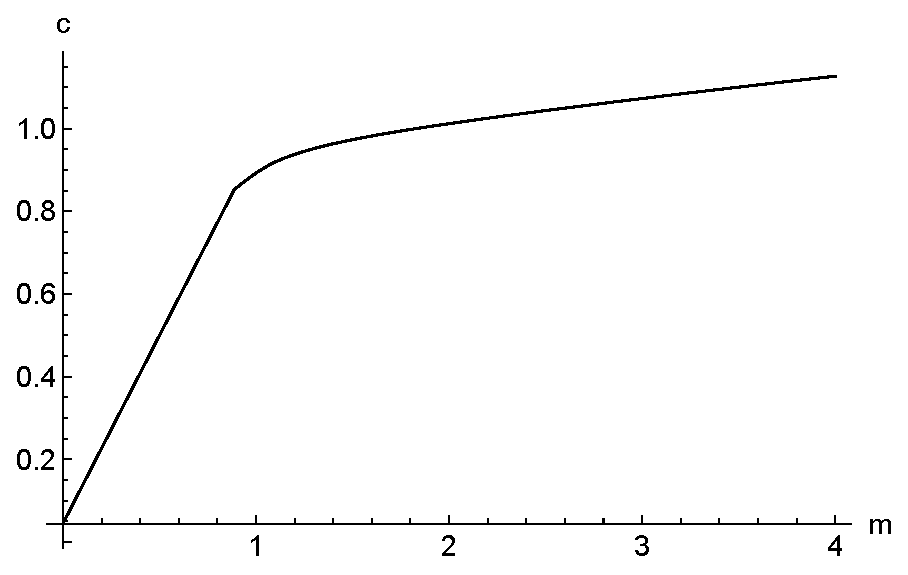
\includegraphics[width=6in]{./Figures/PlotctMultContr}
  \caption{$\cFunc(m_{1})$ With Portfolio Choice}
  \label{fig:PlotctMultContr}
\end{figure}

\hypertarget{PlotRiskySharetOfat}{}
\begin{figure}
  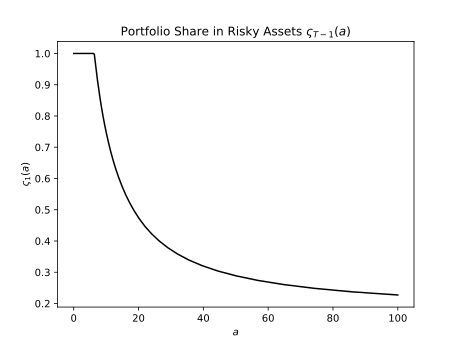
\includegraphics[width=6in]{./Figures/PlotRiskySharetOfat}
  \caption{Portfolio Share in Risky Assets in First Period $\Shr(a)$}
  \label{fig:PlotRiskySharetOfat}
\end{figure}
